\documentclass[tikz,border=4pt]{standalone}
\usepackage{amsmath,amssymb,bm}
\newcommand{\NV}{{N_\mathrm{V}}}
\newcommand{\TD}{{D_\mathrm{T}}}
\usepackage{tikz}
\usetikzlibrary{positioning, arrows.meta}

% Academic executive RGB color palette
\definecolor{cMacro}{RGB}{20, 65, 115}       % Deep Navy
\definecolor{cMacroBg}{RGB}{242, 247, 253}   % Soft Ice Blue
\definecolor{cMicro}{RGB}{15, 95, 85}        % Deep Spruce Teal
\definecolor{cMicroBg}{RGB}{240, 249, 247}   % Soft Mint
\definecolor{cHeur}{RGB}{110, 25, 75}        % Deep Wine
\definecolor{cHeurBg}{RGB}{253, 242, 250}    % Soft Lavender
\definecolor{cPool}{RGB}{165, 75, 10}        % Burnished Amber
\definecolor{cPoolBg}{RGB}{255, 247, 238}    % Soft Warm Cream
\definecolor{cMIP}{RGB}{125, 55, 15}         % Rich Bronze
\definecolor{cMIPBg}{RGB}{252, 243, 236}     % Soft Sand
\definecolor{cArchive}{RGB}{20, 105, 50}     % Forest Green
\definecolor{cArchiveBg}{RGB}{240, 250, 243} % Soft Sage

\begin{document}
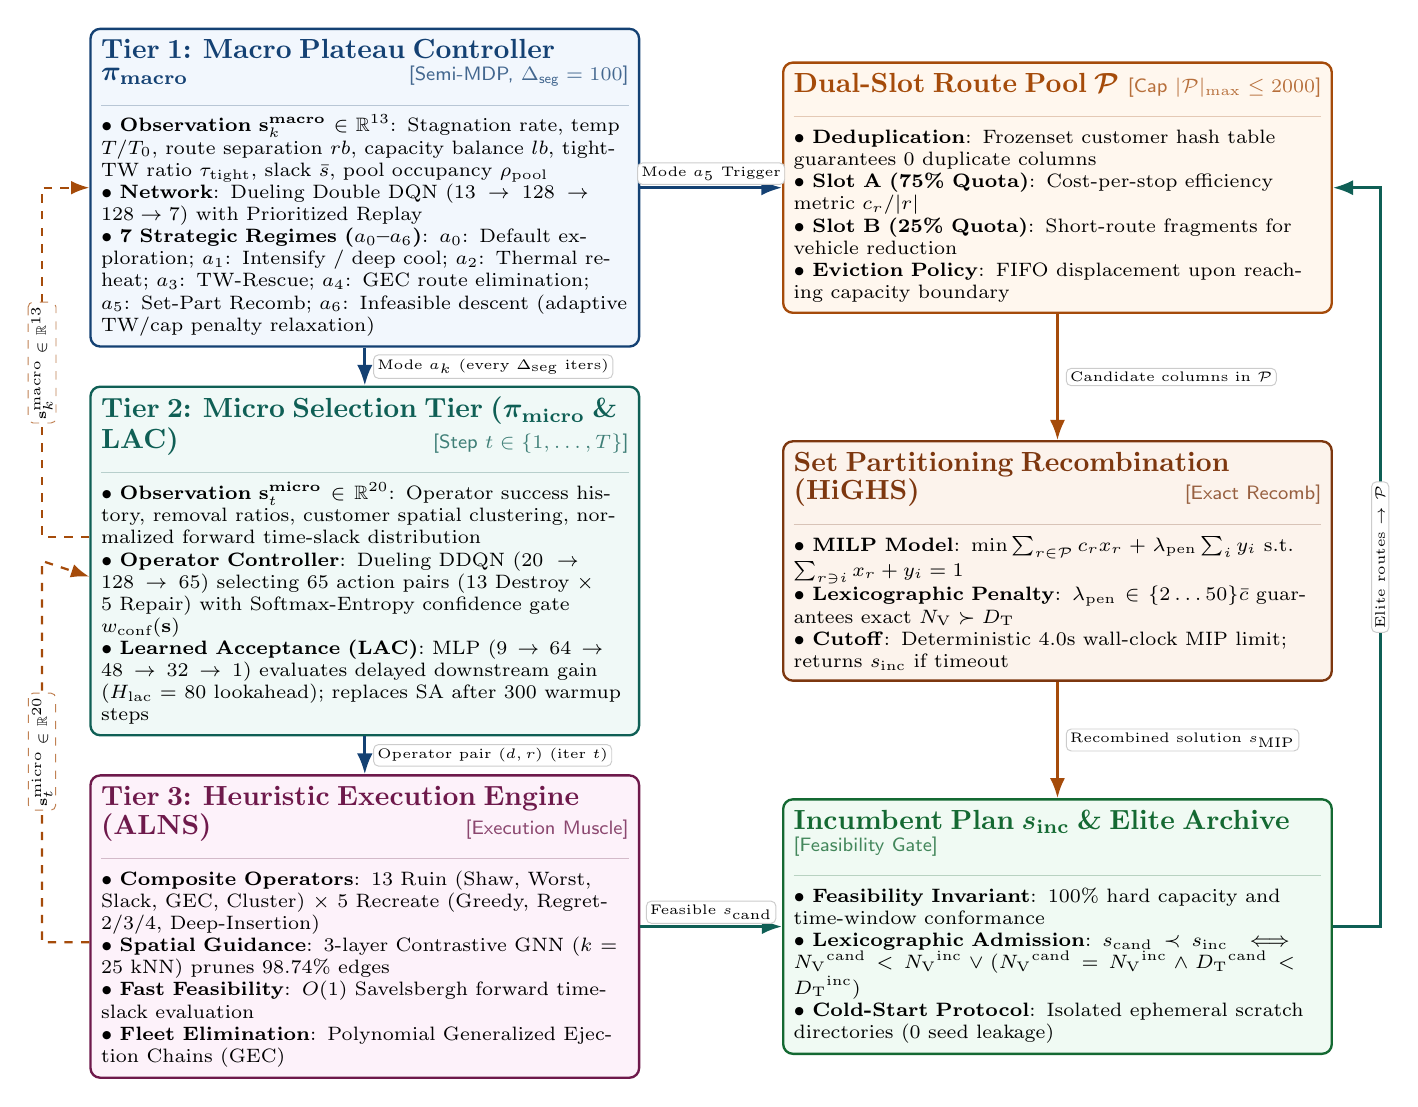
\begin{tikzpicture}[
  >=Latex,
  font=\scriptsize,
  card/.style 2 args={
    draw=#1, fill=#2, rounded corners=3.5pt, line width=0.85pt,
    inner sep=3.8pt, text width=6.7cm, align=left
  },
  rcard/.style 2 args={
    draw=#1, fill=#2, rounded corners=3.5pt, line width=0.85pt,
    inner sep=3.8pt, text width=6.7cm, align=left
  },
  ctrlarr/.style={->, line width=1.0pt, draw=cMacro},
  dataarr/.style={->, line width=0.95pt, draw=cMicro},
  marr/.style={->, line width=0.95pt, draw=cPool},
  fbarr/.style={->, line width=0.8pt, dashed, draw=cPool},
  badge/.style={
    font=\tiny, fill=white, draw=gray!40, line width=0.35pt,
    inner sep=1.4pt, rounded corners=1.8pt
  },
  slopedbadge/.style={
    font=\tiny, fill=white, draw=cPool!70, line width=0.35pt,
    inner sep=1.2pt, rounded corners=1.8pt, sloped, midway
  }
]

  % =========================================================================
  % COLUMN 1: Decision & Search Hierarchy (Tiers 1-3)
  % =========================================================================
  \node[card={cMacro}{cMacroBg}] (macro) {
    {\bfseries\color{cMacro}\normalsize Tier 1: Macro Plateau Controller $\bm{\pi_{\text{macro}}}$}\hfill{\scriptsize\color{cMacro!80}\textsf{[Semi-MDP, $\Delta_{\text{seg}}=100$]}}\\[1pt]
    {\color{cMacro!30}\rule{\linewidth}{0.35pt}}\\[1.5pt]
    $\bullet$ \textbf{Observation $\mathbf{s}_k^{\text{macro}} \in \mathbb{R}^{13}$}: Stagnation rate, temp $T/T_0$, route separation $rb$, capacity balance $lb$, tight-TW ratio $\tau_{\text{tight}}$, slack $\bar{s}$, pool occupancy $\rho_{\text{pool}}$\\
    $\bullet$ \textbf{Network}: Dueling Double DQN ($13 \to 128 \to 128 \to 7$) with Prioritized Replay\\
    $\bullet$ \textbf{7 Strategic Regimes ($a_0$--$a_6$)}: $a_0$: Default exploration; $a_1$: Intensify / deep cool; $a_2$: Thermal reheat; $a_3$: TW-Rescue; $a_4$: GEC route elimination; $a_5$: Set-Part Recomb; $a_6$: Infeasible descent (adaptive TW/cap penalty relaxation)
  };

  \node[card={cMicro}{cMicroBg}, below=4.8mm of macro] (micro) {
    {\bfseries\color{cMicro}\normalsize Tier 2: Micro Selection Tier ($\bm{\pi_{\text{micro}}}$ \& LAC)}\hfill{\scriptsize\color{cMicro!80}\textsf{[Step $t \in \{1,\dots,T\}$]}}\\[1pt]
    {\color{cMicro!30}\rule{\linewidth}{0.35pt}}\\[1.5pt]
    $\bullet$ \textbf{Observation $\mathbf{s}_t^{\text{micro}} \in \mathbb{R}^{20}$}: Operator success history, removal ratios, customer spatial clustering, normalized forward time-slack distribution\\
    $\bullet$ \textbf{Operator Controller}: Dueling DDQN ($20 \to 128 \to 65$) selecting 65 action pairs ($13\text{ Destroy} \times 5\text{ Repair}$) with Softmax-Entropy confidence gate $w_{\text{conf}}(\mathbf{s})$\\
    $\bullet$ \textbf{Learned Acceptance (LAC)}: MLP ($9 \to 64 \to 48 \to 32 \to 1$) evaluates delayed downstream gain ($H_{\text{lac}}=80$ lookahead); replaces SA after 300 warmup steps
  };

  \node[card={cHeur}{cHeurBg}, below=4.8mm of micro] (heur) {
    {\bfseries\color{cHeur}\normalsize Tier 3: Heuristic Execution Engine (ALNS)}\hfill{\scriptsize\color{cHeur!80}\textsf{[Execution Muscle]}}\\[1pt]
    {\color{cHeur!30}\rule{\linewidth}{0.35pt}}\\[1.5pt]
    $\bullet$ \textbf{Composite Operators}: 13 Ruin (Shaw, Worst, Slack, GEC, Cluster) $\times$ 5 Recreate (Greedy, Regret-2/3/4, Deep-Insertion)\\
    $\bullet$ \textbf{Spatial Guidance}: 3-layer Contrastive GNN ($k=25$ kNN) prunes $98.74\%$ edges\\
    $\bullet$ \textbf{Fast Feasibility}: $O(1)$ Savelsbergh forward time-slack evaluation\\
    $\bullet$ \textbf{Fleet Elimination}: Polynomial Generalized Ejection Chains (GEC)
  };

  % =========================================================================
  % COLUMN 2: Recombination & Elite Archive (Right)
  % =========================================================================
  \node[rcard={cPool}{cPoolBg}, right=18mm of macro] (pool) {
    {\bfseries\color{cPool}\normalsize Dual-Slot Route Pool $\bm{\mathcal{P}}$}\hfill{\scriptsize\color{cPool!80}\textsf{[Cap $|\mathcal{P}|_{\max}\le 2000$]}}\\[1pt]
    {\color{cPool!30}\rule{\linewidth}{0.35pt}}\\[1.5pt]
    $\bullet$ \textbf{Deduplication}: Frozenset customer hash table guarantees 0 duplicate columns\\
    $\bullet$ \textbf{Slot A (75\% Quota)}: Cost-per-stop efficiency metric $c_r / |r|$\\
    $\bullet$ \textbf{Slot B (25\% Quota)}: Short-route fragments for vehicle reduction\\
    $\bullet$ \textbf{Eviction Policy}: FIFO displacement upon reaching capacity boundary
  };

  \node[rcard={cMIP}{cMIPBg}, right=18mm of micro] (highs) {
    {\bfseries\color{cMIP}\normalsize Set Partitioning Recombination (HiGHS)}\hfill{\scriptsize\color{cMIP!80}\textsf{[Exact Recomb]}}\\[1pt]
    {\color{cMIP!30}\rule{\linewidth}{0.35pt}}\\[1.5pt]
    $\bullet$ \textbf{MILP Model}: $\min \sum_{r \in \mathcal{P}} c_r x_r + \lambda_{\text{pen}} \sum_{i} y_i$ s.t. $\sum_{r \ni i} x_r + y_i = 1$\\
    $\bullet$ \textbf{Lexicographic Penalty}: $\lambda_{\text{pen}} \in \{2 \dots 50\}\bar{c}$ guarantees exact $\NV \succ \TD$\\
    $\bullet$ \textbf{Cutoff}: Deterministic 4.0s wall-clock MIP limit; returns $s_{\text{inc}}$ if timeout
  };

  \node[rcard={cArchive}{cArchiveBg}, right=18mm of heur] (inc) {
    {\bfseries\color{cArchive}\normalsize Incumbent Plan $\bm{s_{\text{inc}}}$ \& Elite Archive}\hfill{\scriptsize\color{cArchive!80}\textsf{[Feasibility Gate]}}\\[1pt]
    {\color{cArchive!30}\rule{\linewidth}{0.35pt}}\\[1.5pt]
    $\bullet$ \textbf{Feasibility Invariant}: 100\% hard capacity and time-window conformance\\
    $\bullet$ \textbf{Lexicographic Admission}: $s_{\text{cand}} \prec s_{\text{inc}} \iff \NV^{\text{cand}} < \NV^{\text{inc}} \lor (\NV^{\text{cand}} = \NV^{\text{inc}} \land \TD^{\text{cand}} < \TD^{\text{inc}})$\\
    $\bullet$ \textbf{Cold-Start Protocol}: Isolated ephemeral scratch directories (0 seed leakage)
  };

  % =========================================================================
  % VERTICAL DOWNWARD CONTROL & DATA ARROWS
  % =========================================================================
  \draw[ctrlarr] (macro.south) -- node[badge, right=3pt]{Mode $a_k$ (every $\Delta_{\text{seg}}$ iters)} (micro.north);
  \draw[ctrlarr] (micro.south) -- node[badge, right=3pt]{Operator pair $(d,r)$ (iter $t$)} (heur.north);

  \draw[marr] (pool.south) -- node[badge, right=3pt]{Candidate columns in $\mathcal{P}$} (highs.north);
  \draw[marr] (highs.south) -- node[badge, right=3pt]{Recombined solution $s_{\text{MIP}}$} (inc.north);

  % =========================================================================
  % UPWARD STATE FEEDBACK (LEFT FLANK)
  % =========================================================================
  \draw[fbarr] ([yshift=-2mm]heur.west) -- ++(-6mm,0) coordinate (p1)
               -- node[slopedbadge]{$\mathbf{s}_t^{\text{micro}} \in \mathbb{R}^{20}$} (p1 |- micro.west)
               -- ([yshift=-2mm]micro.west);

  \draw[fbarr] ([yshift=3mm]micro.west) -- ++(-6mm,0) coordinate (p2)
               -- node[slopedbadge]{$\mathbf{s}_k^{\text{macro}} \in \mathbb{R}^{13}$} (p2 |- macro.west)
               -- (macro.west);

  % =========================================================================
  % UPWARD ROUTE ACCUMULATION (RIGHT FLANK)
  % =========================================================================
  \draw[dataarr] (inc.east) -- ++(6mm,0) coordinate (p3)
                -- node[badge, midway, sloped]{Elite routes $\to \mathcal{P}$} (p3 |- pool.east)
                -- (pool.east);

  % =========================================================================
  % HORIZONTAL CROSS-TIER ARROWS
  % =========================================================================
  \draw[ctrlarr] (macro.east) -- node[badge, above=1pt]{Mode $a_5$ Trigger} (pool.west);
  \draw[dataarr] (heur.east) -- node[badge, above=1pt]{Feasible $s_{\text{cand}}$} (inc.west);

\end{tikzpicture}
\end{document}
